\subsection{bpmprocess/get\_\-t0.c File Reference}
\label{get__t0_8c}\index{bpmprocess/get\_\-t0.c@{bpmprocess/get\_\-t0.c}}


\subsubsection{Detailed Description}
Declared two helper routines which find the start and end samples for the fit... 

Definition in file {\bf get\_\-t0.c}.

{\tt \#include $<$stdlib.h$>$}\par
{\tt \#include $<$math.h$>$}\par
{\tt \#include $<$bpm/bpm\_\-messages.h$>$}\par
{\tt \#include $<$bpm/bpm\_\-process.h$>$}\par
{\tt \#include $<$bpm/bpm\_\-nr.h$>$}\par


Include dependency graph for get\_\-t0.c:\nopagebreak
\begin{figure}[H]
\begin{center}
\leavevmode
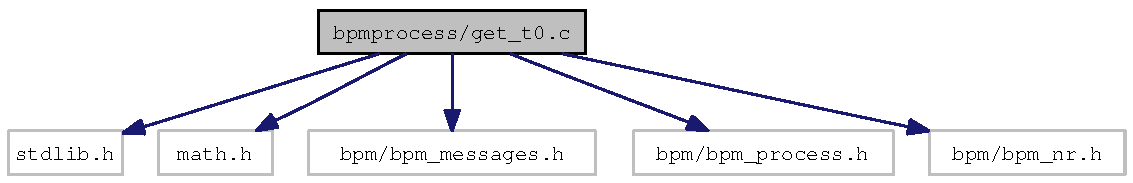
\includegraphics[width=290pt]{get__t0_8c__incl}
\end{center}
\end{figure}
\subsubsection*{Functions}
\begin{CompactItemize}
\item 
void \textbf{\_\-find\_\-t0\_\-startfit} (double $\ast$wf, double ped, int peak\_\-sample, double peak\_\-value, double peak\_\-fraction, int $\ast$start\_\-sample)\label{get__t0_8c_4441082bcc7dd3cf1c46f1dfecc64690}

\item 
void \textbf{\_\-find\_\-t0\_\-endfit} (double $\ast$wf, double ped, int peak\_\-sample, double peak\_\-value, double peak\_\-fraction, int $\ast$end\_\-sample)\label{get__t0_8c_139780fe168b903f9eba5539fb51e5b4}

\item 
int {\bf get\_\-t0} ({\bf doublewf\_\-t} $\ast$signal, double $\ast$t0)
\end{CompactItemize}
